\documentclass[12pt]{article}
\usepackage{fontspec}
 
\setmainfont{Times New Roman}
\setmonofont{Courier New}
\author{Saji Champlin}
\title{CSCI 5204 Homework 1}
\date{}

\usepackage{amsmath}
\usepackage[margin=1in]{geometry}
\usepackage[english]{babel}
\usepackage[shortlabels]{enumitem}
% \usepackage[group-separator={,}]{siunitx}
\usepackage{multicol}
\usepackage{pdfpages}
\usepackage[outputdir=build]{minted}
\usepackage{tikz}
\usepackage{wrapfig}
\usepackage{graphicx}
\usepackage{setspace}
\usepackage{listings}
\usepackage{biblatex}
\addbibresource{refs.bib}
\graphicspath{ {./figures/} }
\usetikzlibrary{patterns}

% minted should always be footnotesize and single spaced.
\setminted{fontsize=\footnotesize,baselinestretch=1, frame=lines, breaklines}

% Don't print section numbers
\setcounter{secnumdepth}{0}

% double space. cursed.
\doublespacing

% disable indentation for new paragraphs.
\setlength{\parindent}{0pt}
\setlength{\parskip}{0pt plus 0.5ex}

\begin{document}
\maketitle

    
\vspace{1cm}

\begin{center}
	\textbf{Abstract}
\end{center}
This project aims to develop a flexible pipelined Fast Fourier Transform (FFT)
that can be adapted to fit any desired data processing pipeline. The pipelined
design means that a new FFT is output on every clock cycle. The design includes
tests for each component of the FFT, including the complex multiplication unit,
and the radix-2 butterfly transform, as well as an example 8-input 16-bit Q8.8
FFT. The design supports arbitrary fixed-point formats, and includes a twiddle
factor ROM that can be generated.

\pagebreak

\section{Preliminary Design Results}
The FFT algorithm is one of the most useful signal processing techniques for
the modern era. It is used from everything for 5G radio modulation to JPEG
compression. This project aims to implement a simple FFT in Verilog for use in
FPGA and ASIC designs.

\subsection{Structure}
FFTs rely on the principle that a DFT can be constructed of two smaller DFTs
that are then combined via a series of radix-2 (radix-4 is also possible but
not used here) "butterfly transforms" that perform complex multiplication with
a "twiddle factor" that rotates the corresponding summations in the complex
domain. A fully realized FFT is then splitting the DFTs until they are reduced
to the base case ($N=2$). The first step to creating the FFT is therefore to
develop a module that can perform complex multiplication with fixed-point
numbers.

\subsubsection{Complex Multiplier}

Verilog has no concept of complex numbers, so we will instead represent them
with two values: the real component and the complex component. Note that for
the pair of complex numbers ($a + bi$,$c +di$), the product is as follows:

\begin{equation*}
	(ac + bd) + (ad + bc)i
\end{equation*}

Meaning that we need to create a custom complex multiplier unit. Furthermore,
the twiddle factors of an FFT are less than 1 in some cases, so we need to use
binary fixed-point numbers to represent them. The advantage with binary fixed
point is that most arithmetic is unchanged, however since multiplication
produces a number that is as wide as the sum of the width of the factors (i.e
two 8-bit numbers when multiplied will never be larger than 16 bits). This
means that our fixed point moves, and so we must be aware of this and get the
correct value when truncating by shifting to the right a certain amount. This
will be explored later in the implementation.

\begin{figure}[H]
	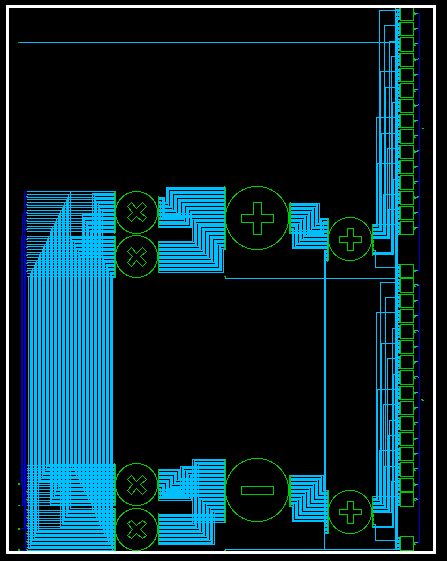
\includegraphics[width=0.7\textwidth]{cplx_schematic.png}
	\centering
	\caption{Schematic for the complex multiplier module}
	\label{fig:cplx_schem}
\end{figure}

\begin{listing}[H]
	\inputminted[frame=lines]{verilog}{../rtl/cplx_mul.v}
\caption{Verilog code for the complex multiplier module}
\label{list:cplx_mul_v}
\end{listing}

The Verilog for this module is quite simple, but there are some key points. The
first is that the inputs, intermediate values, and outputs are all signed. This
is because we are using two's complement notation, and Verilog needs to know
this in order to correctly pad the inputs. The second quirk is the
\texttt{ROUND\_FACTOR} parameter, which is used to increase accuracy when
truncating the output. This trick works by adding 1 to the most significant bit
that will be truncated, causing a carry to occur if it is 1 (if it is 1, it is
closer to the higher value than the lower). Finally, the truncation code is
done with the assign statements. Essentially, we are doubling the position of
the zero point (Q8.8 becomes Q16.16, Q4.12 becomes Q8.24, etc). The bit
selections used ensure that we get the correct bits around the zero-point.


\subsubsection{Butterfly (Radix-2) DFT}
With the complex multiplier complete, we can now construct the base case size-2
DFT, which is often called the butterfly diagram or butterfly transform
\cite{oppenheim1975digital}. The size-2 DFT takes the form as follows:

\begin{align*}
	y_0 &= x_0 + x_1 \\
	y_1 &= x_0 - x_1
\end{align*}

However in addition to this we must apply a multiplicative "twiddle" factor.
The rationale behind this is outside the scope of this document (I don't quite
fully understand it myself). We define a twiddle factor as the complex value
$w_n^k = e^{-2\pi i k / n}$ where $n$ is the number of points, and $k$ is the
part of the transform being computed ($y[k]$) \cite{oppenheim1975digital}.

We then write our modified size-2 DFT as follows:
\begin{align*}
	y_0 &= x_0 + x_1 w_n^k \\
	y_1 &= x_0 - x_1 w_n^k 
\end{align*}

We have the shared product term $x_1 w_n^k$ which we will use the complex
multiplier for. Then the rest of the transform is simple addition and
subtraction.

\begin{figure}[H]
	\centering
	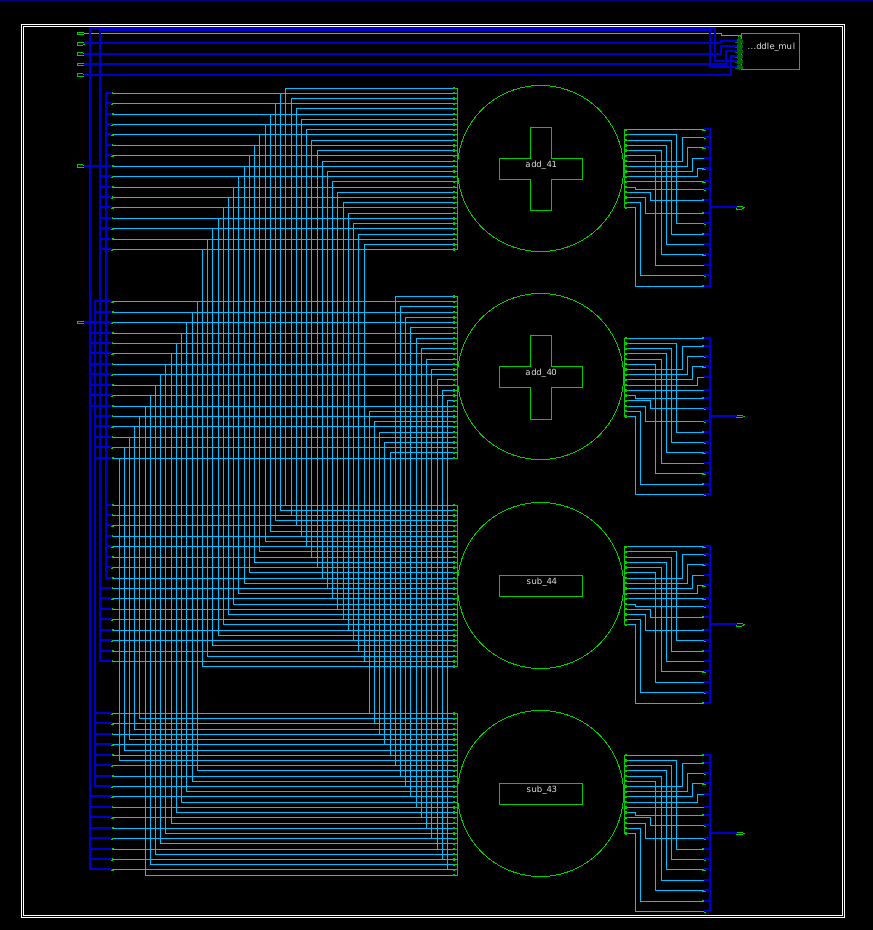
\includegraphics[width=0.7\textwidth]{butterfly_schematic.png}
	\caption{Schematic for the butterfly transform. The module in the upper right is the complex multiplier.}
	\label{fig:butterfly_schem}
\end{figure}

% \begin{listing}[h!]
	\inputminted[frame=lines]{verilog}{../rtl/butterfly.v}
% 	\caption{Verilog code for the butterfly module}
% 	\label{list:butterfly_v}
% \end{listing}
Note that this design uses a combinatorial always block, to prevent needing two
clocks to get the correct value.
\pagebreak
\subsubsection{FFT-8 example (incomplete)}

\begin{figure}[h]
	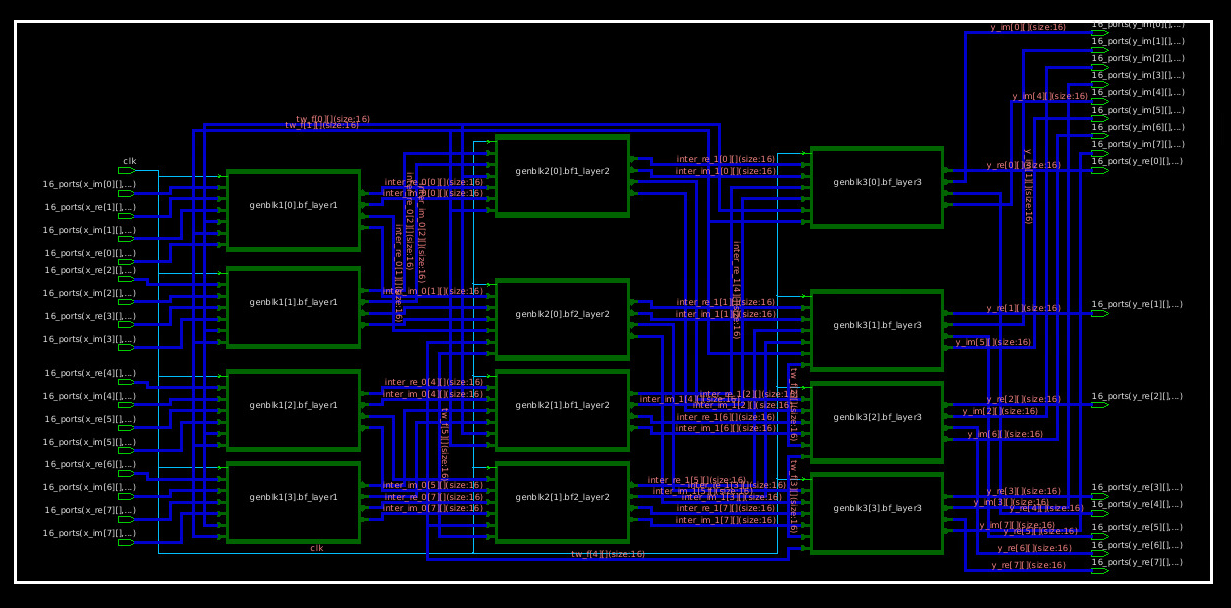
\includegraphics[width=\textwidth]{fft_schematic.png}
	\caption{8-Point FFT schematic (incomplete)}
	\label{fig:fft_schem}
\end{figure}
The only thing remaining to do is to instantiate the butterfly transforms
in the correct layout, with twiddle factors loaded in as well. I was not able
to get this module working at this time, with strange behavior on the
simulator. There is also a bit-reversal component which I have not implemented
yet. Figure~\ref{fig:fft_schem} shows the current schematic for the demo
8-point FFT. Below is the listing for the FFT. Note the extensive use of
generate blocks. It is my hope that I will be able to largely automate
the design using some Python and Verilog parameters, to allow for
scaling to fit various applications.

% \begin{listing}[h!]
	\inputminted[frame=lines]{verilog}{../rtl/fft.v}
% 	\caption{Verilog code for the demo FFT module}
% 	\label{list:fft_v}
% \end{listing}

\subsection{Simulation}

For simulation and testing of the FFT, I opted to use a relatively new tool
called \texttt{cocotb}\cite{cocotb}, which is a Python library that can interface directly
with a variety of synthesis tools, such as Synopsys VCS, Cadence XCelium, and
Icarus Verilog. My reasoning for this was twofold. The first is that I would
like to be able to run the test suites for this design after I no longer have
access to commercial tools (no need to write TCL scripts to validate outputs).
The second reason is that I can more easily code complex behavior in python.
For example, my complex multiplier test suite has some known-good values, but
also runs through 1000 randomly generated complex number pairs and compares the
expected value (calculated in python) to the output of the simulator. This
was a little tricky to set up due to fixed point rounding, but was far easier
to get running than alternatives I believe.

An example test case for the complex multiplier looks like the following:

\begin{minted}{python}
@cocotb.test()
async def test_cplx(dut):
    cocotb.start_soon(Clock(dut.clk, 1, 'ns').start())

    await set_terms(dut, 2 + 1j, 3 + 4j) #set input values
    await RisingEdge(dut.clk) #clock it in
    await ReadWrite() # wait for the values to propagate.
    res = await get_product(dut) # get output, convert to python complex
    assert res == 2 + 11j

\end{minted}

\texttt{set\_terms} and \texttt{get\_product} are helper functions that format the
bits and convert it to Python data types for input and output respectively. 
Running the test suite produces an output like:

\begin{minted}{c}
******************************************************************
** TEST                                  STATUS  SIM TIME (ns)  **
******************************************************************
** tests.test_cplx_mul.test_unity         PASS           1.00   **
** tests.test_cplx_mul.test_negation      PASS           1.00   **
** tests.test_cplx_mul.test_imag          PASS           1.00   **
** tests.test_cplx_mul.test_cplx          PASS           1.00   **
** tests.test_cplx_mul.test_rand_ints     PASS         100.00   **
** tests.test_cplx_mul.test_rand_floats   PASS        1000.00   **
******************************************************************
** TESTS=6 PASS=6 FAIL=0 SKIP=0                       1104.01   **
******************************************************************
\end{minted}
The test suite includes random tests for both pure integers and floating point
numbers that are converted to fixed point. 


I used Icarus Verilog for most of my testing. Before I finish the project,
I would like to check that \texttt{cocotb} works with VCS and XCelium on lab
machines. I had Icarus output the waveforms for the complex multiplier to a vcd
file to visually inspect them using GtkWave:

\begin{figure}[H]
	\centering
	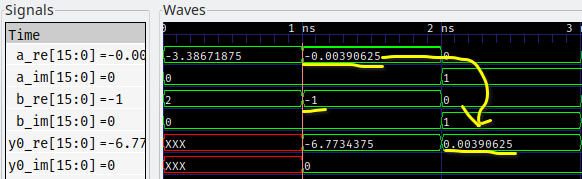
\includegraphics[width=0.7\textwidth]{cplx_mul_waveform.png}
	\caption{Waveform of simple operation of complex multiplier.}
	\label{fig:waveform}
\end{figure}
Here the test bench is just attempting to negate the result, and on the next
clock cycle, we can see that it was successful.

\subsection{Layout}
The layout of this design is concerning due to the large amount of wide
arithmetic needed to achieve a good result. The most notable part is the
1-clock multipliers, which are incredibly large devices. To get a rough idea of
how much area is needed, I synthesized a complex multiplier from start to
finish using a modified version of the design compiler TCL flow. I did not
specify any timing constraints beyond a 2 nanosecond clock period.

Below are the power, area, and timing reports for a single complex multiplier
with default parameters: 16 bit wide inputs (32 bits total because of real and
imaginary), and a fixed point at 8 bits using none of the advanced
optimizations outlined in later labs.

\begin{minted}[fontsize=\scriptsize]{c}
Information: report_power power group summary does not include estimated clock tree power. (PWR-789)
                 Internal         Switching           Leakage            Total                         Cell
Power Group      Power            Power               Power              Power   (   %    )  Attrs  Count
---------------------------------------------------------------------------------------------------------
io_pad             0.0000            0.0000            0.0000            0.0000  (   0.00%)            0
memory             0.0000            0.0000            0.0000            0.0000  (   0.00%)            0
black_box          0.0000            0.0000            0.0000            0.0000  (   0.00%)            0
clock_network      0.0000            0.0000            0.0000            0.0000  (   0.00%)            0
register           0.0000            0.0000            0.0000            0.0000  (   0.00%)            0
sequential        25.0948            0.1005        2.0997e+06           27.2950  (   1.99%)            32
combinational    981.1514          356.8938        8.4837e+06        1.3465e+03  (  98.01%)            2054
---------------------------------------------------------------------------------------------------------
Total          1.0062e+03 uW       356.9944 uW     1.0583e+07 pW     1.3738e+03 uW
\end{minted}

\begin{minted}{c}
Number of ports:                          100
Number of nets:                          2761
Number of cells:                         2087
Number of combinational cells:           2054
Number of sequential cells:                32
Number of macros/black boxes:               0
Number of buf/inv:                        371
Number of references:                      32

Combinational area:               5936.041318
Buf/Inv area:                      477.282434
Noncombinational area:             292.773895
Macro/Black Box area:                0.000000
Net Interconnect area:            1693.132825

Total cell area:                  6228.815213
Total area:                       7921.948038
\end{minted}

\newpage
\section{Conclusion}

At this point, I am fairly confident in the design of the complex multiplier
and butterfly DFT unit being functionally correct. There are issues with the
FFT module, namely that it only seems to output zeros past the first stage. I
will need to debug this in greater depth to understand why this is happening.
Furthermore, there's one module that I forgot to implement, and that is a
bit-reversal stage on the input. I'm still reading up on why this is necessary.

The most obvious next step is to get the design fully working, and finish
my FFT test suite. As mentioned, there are missing parts, and there are
also probably incorrect interconnections in the top module or some other
human error. The test suites for the sub modules are fairly robust and
have yet to fail once I had a green board. VCS might be nice here for coverage
reports, but I'm not sure how fine-grained those can get (I would like to test
that every bit on a wire is correct). Since I have tested the butterfly unit
pretty intensely, I'm convinced that the error is some implementation detail
that's missing on the top module

Next, I will need to do a lot more work in the layout once the FFT itself
is working in the simulator. My hope is that most of the optimizations (for
example, only supporting real-valued input sequences) will be automatic, but
I could see there being other issues. One challenge is that the synthesis
process starts to slow down with more complex designs. The complex multiplier
shown above took four minutes to compile everything. If time allows, I would
also like to apply some of the techniques used in later labs to improve
the specs of the layout.

Finally, if I can get the layout into a good state, I would like to push for an
automated verilog generator with a Python script. I don't think it would be
easy to generate N-sized FFTs in pure Verilog, but I can use parameters for 
things like bit-width and fixed point location. I could go one step further
and then generate a specialized test suite for that particular FFT, but I would
probably want more Python libraries like NumPy to help me out then.


\newpage
\printbibliography


\end{document}
